%%%%%%%%%%%%%%%%%%%%%%%%%%%%%%%%%%%%%%%%%
% Beamer Presentation
% LaTeX Template
% Version 1.0 (10/11/12)
%
% This template has been downloaded from:
% http://www.LaTeXTemplates.com
%
% License:
% CC BY-NC-SA 3.0 (http://creativecommons.org/licenses/by-nc-sa/3.0/)
%
%%%%%%%%%%%%%%%%%%%%%%%%%%%%%%%%%%%%%%%%%

%----------------------------------------------------------------------------------------
%	PACKAGES AND THEMES
%----------------------------------------------------------------------------------------

\documentclass{beamer}

\mode<presentation> {

% The Beamer class comes with a number of default slide themes
% which change the colors and layouts of slides. Below this is a list
% of all the themes, uncomment each in turn to see what they look like.

%\usetheme{default}
%\usetheme{AnnArbor}
%\usetheme{Antibes}
%\usetheme{Bergen}
%\usetheme{Berkeley}
%\usetheme{Berlin}
%\usetheme{Boadilla}
%\usetheme{CambridgeUS}
%\usetheme{Copenhagen}
%\usetheme{Darmstadt}
\usetheme{Dresden}
%\usetheme{Frankfurt}
%\usetheme{Goettingen}
%\usetheme{Hannover}
%\usetheme{Ilmenau}
%\usetheme{JuanLesPins}
%\usetheme{Luebeck}
%\usetheme{Madrid}
%\usetheme{Malmoe}
%\usetheme{Marburg}
%\usetheme{Montpellier}
%\usetheme{PaloAlto}
%\usetheme{Pittsburgh}
%\usetheme{Rochester}
%\usetheme{Singapore}
%\usetheme{Szeged}
%\usetheme{Warsaw}

% As well as themes, the Beamer class has a number of color themes
% for any slide theme. Uncomment each of these in turn to see how it
% changes the colors of your current slide theme.

%\usecolortheme{albatross}
%\usecolortheme{beaver}
%\usecolortheme{beetle}
%\usecolortheme{crane}
%\usecolortheme{dolphin}
%\usecolortheme{dove}
%\usecolortheme{fly}
%\usecolortheme{lily}
%\usecolortheme{orchid}
%\usecolortheme{rose}
%\usecolortheme{seagull}
%\usecolortheme{seahorse}
%\usecolortheme{whale}
%\usecolortheme{wolverine}

%\setbeamertemplate{footline} % To remove the footer line in all slides uncomment this line
%\setbeamertemplate{footline}[page number] % To replace the footer line in all slides with a simple slide count uncomment this line

%\setbeamertemplate{navigation symbols}{} % To remove the navigation symbols from the bottom of all slides uncomment this line
}

\usepackage{graphicx} % Allows including images
\usepackage{booktabs} % Allows the use of \toprule, \midrule and \bottomrule in 
%tables
\usepackage{listings}

%----------------------------------------------------------------------------------------
%	TITLE PAGE
%----------------------------------------------------------------------------------------

\title[Lecture 2]{Advanced R Programming - Lecture 2} % The short title 
%appears at the bottom of every slide, the full title is only on the title page

\author{Leif Jonsson} % Your name
\institute[STIMA LiU] % Your institution as it will appear on the bottom of 
%every 
%slide, may be shorthand to save space
{
Link\"{o}ping University \\ % Your institution for the title page
\medskip
\textit{leif.jonsson@ericsson.com\\leif.r.jonsson@liu.se} % Your email address
}
\date{\today} % Date, can be changed to a custom date

\begin{document}

\begin{frame}
\titlepage % Print the title page as the first slide
\end{frame}

\begin{frame}
\frametitle{Today} % Table of contents slide, comment this block out to remove 
%it
\tableofcontents % Throughout your presentation, if you choose to use \section{} and \subsection{} commands, these will automatically be printed on this slide as an overview of your presentation
\end{frame}

%----------------------------------------------------------------------------------------
%	PRESENTATION SLIDES
%----------------------------------------------------------------------------------------

\begin{frame}
	\Huge{\centerline{Questions since last time?}}
\end{frame}

%------------------------------------------------
\section{Program Control} % Sections can be created in order to organize your 
%presentation into discrete blocks, all sections and subsections are 
%automatically printed in the table of contents as an overview of the talk
%------------------------------------------------

\begin{frame}
\frametitle{Program Control}
Two main components
\begin{itemize}
\item Conditional statements
\item Loops
\end{itemize}
See also extra video on program control on course page
\end{frame}

\defverbatim[colored]\lstCond{
	\begin{lstlisting}[language=R,basicstyle=\ttfamily,keywordstyle=\color{red},
	basicstyle=\small]
	if(boolean expression) {
	# commands
	} else if (boolean expression) {
	# commands
	} else {
	# commands
	}
	\end{lstlisting}
}

\begin{frame}
	\frametitle{Conditional statements}
	\lstCond
\end{frame}

\begin{frame}
	\frametitle{Loops}
	\begin{itemize}
		\item for
		\item while
		\item repeat
	\end{itemize}
	See also extra video on program control on course page
\end{frame}

\defverbatim[colored]\lstFor{
	\begin{lstlisting}[language=R,basicstyle=\ttfamily,keywordstyle=\color{red},
	basicstyle=\small]
	for (name in vector){
	# statements
	}
	\end{lstlisting}
}

\begin{frame}
	\frametitle{For loop}
	\lstFor
\end{frame}

\defverbatim[colored]\lstWhile{
	\begin{lstlisting}[language=R,basicstyle=\ttfamily,keywordstyle=\color{red},
	basicstyle=\small]
	while (boolean expression){
	# statements
	}
	\end{lstlisting}
}

\begin{frame}
	\frametitle{While loop}
	\lstWhile
\end{frame}

\defverbatim[colored]\lstRepeat{
	\begin{lstlisting}[language=R,basicstyle=\ttfamily,keywordstyle=\color{red},
	basicstyle=\small]
	repeat {
	# statements
	}
	\end{lstlisting}
}

\begin{frame}
	\frametitle{Repeat loop}
	\lstRepeat
\end{frame}


\begin{frame}
	\frametitle{Controlling loops}
		\begin{itemize}
			\item break (loop)
			\item next (iteration)
		\end{itemize}
\end{frame}

%------------------------------------------------
\section{Functions}
%------------------------------------------------

\defverbatim[colored]\lstFun{
	\begin{lstlisting}[language=R,basicstyle=\ttfamily,keywordstyle=\color{black},
	basicstyle=\small]
	my_function_name <- function(x, y){
	  z <- x^2 + y^2
	  return(z)
	}
	\end{lstlisting}
}

\begin{frame}
	\frametitle{Functions revisited}
	\lstFun
\end{frame}

\begin{frame}
	\frametitle{Function components}
	Function arguments \\
	Function body \\
	Function environment \\~\\

	These can be accessed in R by: \\
	formals(f) \\
	body(f) \\
	environment(f)	
\end{frame}


%------------------------------------------------
\section{Environments and scoping}
%------------------------------------------------

\begin{frame}
	\frametitle{Lexical scoping}
	\centerline{(or how do R find stuff?)}
	\begin{center}
		Current environment $\Rightarrow$ \\
		Parent environment $\Rightarrow$ \\
		... \\
		Global environment $\Rightarrow$ \\
		... along searchpath to... \\
		Empty environment (fail)
	\end{center}
\end{frame}

\begin{frame}
	\frametitle{Environment search path}
	\begin{figure}[!ht]
		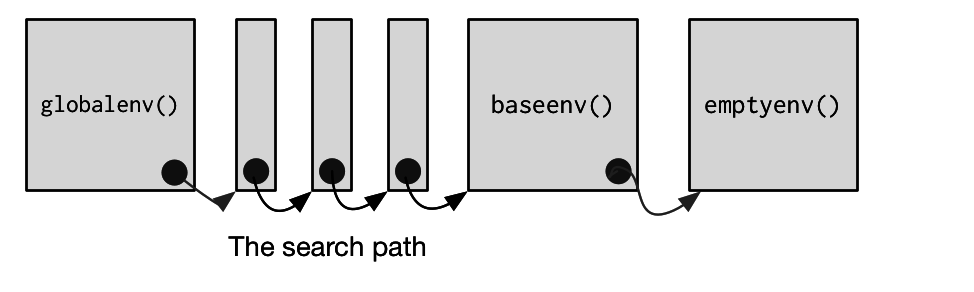
\includegraphics[scale=0.90]{figures/search-path}
		\caption{Environment search-path}
		\label{fig:enviii}
	\end{figure}
\end{frame}

\defverbatim[colored]\lstEnvI{
	\begin{lstlisting}[language=R,basicstyle=\ttfamily,keywordstyle=\color{black},
	basicstyle=\small]
	e <- new.env()
	e$a <- FALSE
	e$b <- "a"
	e$c <- 2.3
	e$d <- 1:3
	\end{lstlisting}
}

\begin{frame}
	\frametitle{Environment basics}
	"bag of names"
	\lstEnvI
	\begin{figure}[!ht]
		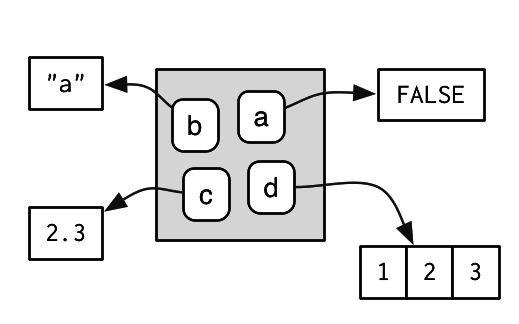
\includegraphics[scale=0.90]{figures/bindingsenv}
		\caption{Environment}
		\label{fig:envi}
	\end{figure}
\end{frame}

\begin{frame}
	\frametitle{Environment relatives}
	\centerline{Parents, but no children}
	\begin{figure}[!ht]
		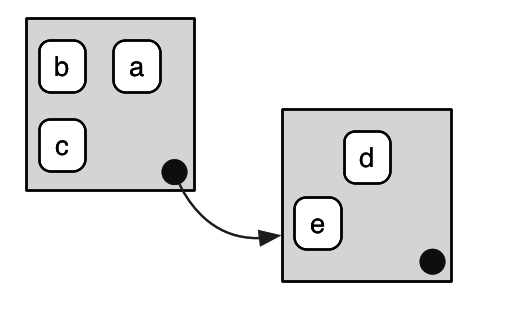
\includegraphics[scale=0.90]{figures/parents}
		\caption{Env. relations}
		\label{fig:envii}
	\end{figure}
\end{frame}

\begin{frame}
	\frametitle{Working with environments}
	\begin{center}	
		See environments as lists \\~\\
		\texttt{ls()}
	\end{center}
\end{frame}

\begin{frame}
	\frametitle{Assignments}
	\begin{center}
		Shallow assignment \\
		$\textless-$ \\~\\
		Deep assignment \\
		$\textless\textless-$ \\~\\
		Full control assignment \\
		\texttt{assign()} \\
	\end{center}
\end{frame}

%------------------------------------------------
\section{Function arguments}
%------------------------------------------------

\begin{frame}
	\frametitle{Function arguments}
	\centerline{copy-on-modify semantics}
	\begin{center}
		specify arguments by... \\~\\
		position \\
		complete name \\
		partial name \\
	\end{center}
\end{frame}


\begin{frame}
	\frametitle{Function arguments (cont)}
	\centerline{copy-on-modify semantics}
	\begin{center}
		\texttt{do.call()} \\
		\texttt{missing()} \\
		... \\
		Default values \\
	\end{center}
\end{frame}

%------------------------------------------------
\section{Returning values}
%------------------------------------------------

\begin{frame}
	\frametitle{Return values}
	\begin{center}
		The last expression evaluated in a function \\
		Multiple values using lists \\
		Pure functions \\~\\
		
		on.exit() \\
		
		return()
	\end{center}
\end{frame}


%------------------------------------------------
\section{Specials}
%------------------------------------------------

\begin{frame}
	\frametitle{Specials}
	\begin{center}
		infix functions \\
		replacement functions \\
	\end{center}
\end{frame}

%------------------------------------------------
\section{Functionals}
%------------------------------------------------

\begin{frame}
	\frametitle{Functionals}
	\begin{center}
		Higher order functions \\
		Common in mathematics and functional languages\\
	\end{center}
\end{frame}


\begin{frame}
	\frametitle{Functionals}
	\centerline{Pros}
	\begin{center}
		(Often) faster alt. to loops \\
		Easy to parallelize \\
		Encourages you to think about independence (see above point)
	\end{center}
\end{frame}

\begin{frame}
	\frametitle{Functionals}
	\centerline{Cons}
	\begin{center}
		Can't handle serially dependent algorithms \\
		Can make code more difficult to read
	\end{center}
\end{frame}

\begin{frame}
	\frametitle{Common Functionals}
	\begin{center}
		\texttt{lapply()} \\
		\texttt{vapply()} \\
		\texttt{sapply()} \\
		\texttt{apply()} \\
		\texttt{tapply()} \\
		\texttt{mapply()} \\
	\end{center}
\end{frame}

%------------------------------------------------
\section{Functional programming}
%------------------------------------------------

\begin{frame}
	\frametitle{Functional programming}
	\begin{center}
		Programming paradigm \\
		Foundation in R
	\end{center}
\end{frame}

\begin{frame}
	\frametitle{Anonymous functions}
	\begin{center}
		Functions without names \\
		Often used in functionals
	\end{center}
\end{frame}


\begin{frame}
	\frametitle{Closures}
	\begin{center}
		''An object is data with functions. A closure is a function with 
		data.'' \\ 
		— John D. Cook
	\end{center}
\end{frame}

\defverbatim[colored]\lstClosure{
	\begin{lstlisting}[language=R,basicstyle=\ttfamily,keywordstyle=\color{black},
	basicstyle=\small]
	counter_factory <- function(){
	  i <- 0
	  f <- function(){
	    i <<- i + 1
	    i
	  }
	  f
	}
	
	first_counter <- counter_factory()
	second_counter <- counter_factory()
	
	first_counter()
	first_counter()
	second_counter()
	
	ls(environment(first_counter))
	environment(first_counter)$i
	\end{lstlisting}
}

\begin{frame}
	\frametitle{Closure example}
	\lstClosure
\end{frame}

%------------------------------------------------
\section{R packages}
%------------------------------------------------

\begin{frame}
	\frametitle{R packages}
	\begin{center}
		An environment with functions and/or data \\
		The way to share code and data \\~\\
		~4 000 developers \\
		\textgreater 7000 package \\
	\end{center}
\end{frame}

\begin{frame}
	\frametitle{Package basics}
	\begin{center}
		Usage \\
		\texttt{library()} \\
		\texttt{::} \\
		\texttt{:::} \\~\\
		Installation \\
		\texttt{install.packages()} \\
		\texttt{devtools::install\_github()} \\
		\texttt{devtools::install\_local()} \\
	\end{center}
\end{frame}

\begin{frame}
	\frametitle{Package namespace}
	\begin{center}
			\begin{figure}[!ht]
				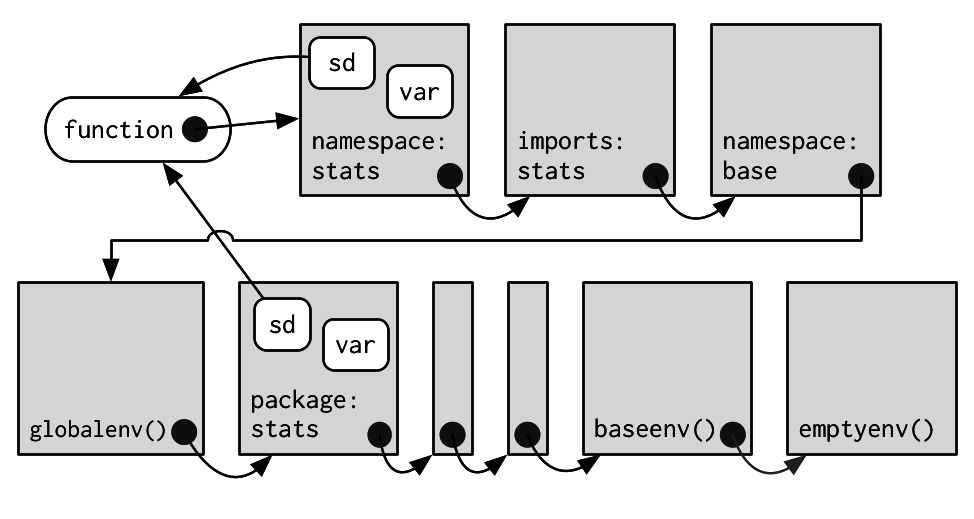
\includegraphics[scale=0.90]{figures/namespace}
				\caption{Package namespace}
				\label{fig:pkgns}
			\end{figure}
	\end{center}
\end{frame}

\begin{frame}
	\frametitle{Which are good packages}
	\centerline{Examine the package}
	\begin{center}
		\begin{enumerate}
			\item Who?			
			\item When updated?			
			\item In development?
		\end{enumerate}
	\end{center}
\end{frame}

\begin{frame}
	\frametitle{Semantic versioning}
	\begin{center}
	''Dependency hell'' \\~\\
	\texttt{[MAJOR].[MINOR].[PATCH]} \\~\\
	(See reference on course page)
	\end{center}
\end{frame}

%------------------------------------------------

\begin{frame}
\Huge{\centerline{The End... for today.}}
\Huge{\centerline{Questions?}}
\Huge{\centerline{See you next time!}}
\end{frame}

%----------------------------------------------------------------------------------------

\end{document} 